\subsection{Grafcet Máquina 7 embalaje}
Esta máquina (\hyperref[graf:maq7]{Máquina 7, embalaje}) es similar a la máquina 5 de la línea de soportes (\hyperref[sec:map5_sop]{Sección de la Máquina 5 de Soportes}). Se cuenta el número de piezas embaladas para, al alcanzar el cupo, levantar el clamper y mover la caja a otra zona.
 
\begin{figure}[H]
	\centering
	\includegraphics[width=0.8\linewidth]{./Figuras/maq7_EMB.png}
	\medskip
	\label{fig:maq7_emb}
	\caption{Máquina 7 de la línea de embalaje}
\end{figure}

\begin{figure}[H]
	\centering
	\scalebox{0.75}{%\nodeDist = 2.5cm
%\retornoDist = 0.7\nodeDist % Distància vertical dels retorns
%\bifDistX = 10ex
%\bifDistY = 1.1\nodeDist
%\sincDistYabove = 0.85\nodeDist
%\sincDistYbelow = 0.6\sincDistYabove
%\sincDistYBlockbelow = 0.5\nodeDist


\begin{tikzpicture}[auto]
	
	\ttfamily
	
% --------------------------------------------
	\ttfamily
	
	\etapaInicial{100}
	\primeraAccion{100}{X100-A1}{MAQ\_LIBRE}
    \otraAccion{X100-A1}{X100-A2}{$\mathtt{C:=0}$}
  \sobreActivacion{X100-A2}{X100-A3}{}
	%---

	\etapa[1.25\nodeDist]{101}{100}{Act\_Maq};
	\primeraAccion{101}{X101-A1}{QC7}
	
	%--
	\etapa[1.25\nodeDist]{102}{101}{S5};
	\primeraAccion{102}{X102-A1}{QC7}

	%---
	\etapa[1.25\nodeDist]{103}{102}{1s/X102};
	\primeraAccion{103}{X103-A1}{QCLAMP}

	\etapa[1.25\nodeDist]{104}{103}{1s/X103};
	\primeraAccion{104}{X104-A1}{HAYSPieza}

  \etapa[1.25\nodeDist]{105}{104}{Pieza\_Empaquetada};
  \primeraAccion{105}{X105-A1}{$\mathtt{C:=C+1}$}
  \sobreActivacion{X105-A1}{X105-A2}{}

  %\retornoInicio[-10em]{105}{104}{$\mathtt{C<2}$}
  %\etapa[1.25\nodeDist]{104}{105}{$\mathtt{C<2}$}
  \saltoHorizontal[5.5cm]{105}{104}{$\mathtt{C<2}$}
  
  \etapa[1.4\nodeDist]{106}{105}{$\mathtt{C==1}$};
	\primeraAccion{106}{X106-A1}{QCLAMP\_SUB}
	\otraAccion{X106-A1}{X106-A2}{QC7}

  \etapa[1.25\nodeDist]{107}{106}{3s/X106};
	\primeraAccion{107}{X107-A1}{Pieza\_Entregada}
	
	

	\retornoInicio[6em]{107}{0}{\underline{1}}
	
       
\end{tikzpicture}}
	\medskip
	\caption{Grafcet de la Máquina 7 embalaje}
	\label{graf:maq7}
\end{figure}

\subsection{Grafcet de Mantenimiento}
El \hyperref[graf:mantenimiento]{Grafcet de Mantenimiento}
 asegura que la máquina funciona correctamente antes de procesar
 lotes. Se ejecuta al arrancar la máquina y después de la ejecución
  del \hyperref[graf:principal_vaciado]{Grafcet Principal de Vaciado},
   garantizando que la puesta en marcha tras soltar la seta sea
    correcta.

	Dispone tamibién de un botón en la pantalla de configuración del HMI
	(\ref{fig:HMI_config}) para que un 
	usuario con permisos pueda activarlo
	en cualquier momento.

\begin{figure}[H]
	\centering
	\scalebox{0.75}{%\nodeDist = 2.5cm
%\retornoDist = 0.7\nodeDist % Distància vertical dels retorns
%\bifDistX = 10ex
%\bifDistY = 1.1\nodeDist
%\sincDistYabove = 0.85\nodeDist
%\sincDistYbelow = 0.6\sincDistYabove
%\sincDistYBlockbelow = 0.5\nodeDist


\begin{tikzpicture}[auto]
	
	\ttfamily
	
	\etapaInicial{110}
	
	%---
	\etapa[1.25\nodeDist]{111}{110}{Act\_Mantenimiento};

	
	%--
	\etapa[1.25\nodeDist]{112}{111}{\NOT{SENSORES}};
	\primeraAccion{112}{X112-A1}{Activar\_Cinta}
	
	%---
	\etapa[1.25\nodeDist]{113}{112}{2s/X112};
	\primeraAccion{113}{X113-A1}{Activar\_Transfers}

	\etapa[1.25\nodeDist]{114}{113}{2s/X113};
	\primeraAccion{114}{X114-A1}{Bajar\_Robot}
  \otraAccion{X114-A1}{X114-A2}{Subir\_CLAMPER}

	\etapa[1.25\nodeDist]{115}{114}{2s/X114};
	\primeraAccion{115}{X115-A1}{Grippers}
  \otraAccion{X115-A1}{X115-A2}{CLAMPER}

	\etapa[1.25\nodeDist]{116}{115}{2s/X115};
	\primeraAccion{116}{X116-A1}{Mover\_Horizontal\_Robots}

  \etapa[1.25\nodeDist]{117}{116}{2s/X116};
	\primeraAccion{117}{X117-A1}{Fin\_Mantenimiento}

	\retornoInicio[6em]{117}{0}{\underline{1}}

\end{tikzpicture}
}
	\medskip
	\caption{Grafcet de Mantenimiento}
	\label{graf:mantenimiento}
\end{figure}

\subsection{Grafcet Principal de Vaciado}
El \hyperref[graf:principal_vaciado]{Grafcet Principal de Vaciado}
 se activa tras desenclavar la seta de emergencia, 
 ya que no se aceptan las piezas que
  estuvieran en la máquina durante la emergencia.
   Las máquinas también se pueden vaciar 
   si un usuario con permisos pulsa el botón
    de vaciado del HMI (\ref{fig:HMI_config}).

\begin{figure}[H]
	\centering
	\scalebox{0.75}{\begin{tikzpicture}
  \ttfamily

  %---------------------------
  % Columna izquierda
  %---------------------------
  \etapaInicial{120}
  \etapa[1.25\nodeDist]{121}{120}{VACIAR\_MAQS};
  \primeraAccion{121}{X121-A1}{Activar\_Vaciado\_Maquinas}
  
 
  
  
  \etapa[1.25\nodeDist]{122}{121}{Fin\_VAC\_VAC\_1 $\cdot$ Fin\_VAC\_EMB\_1 $\cdot$ Fin\_VAC\_SOP\_1 $\cdot$ Fin\_VAC\_VAC\_2 $\cdot$ Fin\_VAC\_EMB\_2 $\cdot$ Fin\_VAC\_SOP\_2 };
 	\primeraAccion{122}{X122-A1}{Fin\_Vaciado}
  
    \etapa[1.25\nodeDist]{122V2}{122}{ $\cdot$ Fin\_VAC\_VAC\_3 $\cdot$ Fin\_VAC\_EMB\_3 $\cdot$ Fin\_VAC\_SOP\_3 $\cdot$ Fin\_VAC\_SOP\_4};
 	\primeraAccion{122V2}{X122V2-A1}{Fin\_Vaciado}

  \retornoInicio[6cm]{122V2}{120}{\underline{1}}






  


\end{tikzpicture}
}
	\medskip
	\caption{Grafcet Principal de Vaciado}
	\label{graf:principal_vaciado}
\end{figure}

\subsection{Grafcet vaciado tipo 1}
 \subsubsection{Grafcet Vaciado 1}
 
 El \hyperref[graf:vaciado_1]{Grafcet de Vaciado 1} se 
 activa por medio del \hyperref[graf:principal_vaciado]{Grafcet Principal de Vaciado}, 
 y este vacía las siguientes máquinas:
\begin{itemize}
	\item Máquina 1:
	\begin{itemize}
		\item \hyperref[fig:maq1]{Vacunas, Soportes y Embalajes}
	\end{itemize}
	\item Máquina 2:
	\begin{itemize}
		\item \hyperref[fig:maq2]{Vacunas, Soportes y Embalajes}
	\end{itemize}
	\item Máquina 3:
	\begin{itemize}
		\item \hyperref[fig:maq3]{Vacunas, Soportes y Embalajes}
	\end{itemize}
	\item Máquina 4:
	\begin{itemize}
		\item \hyperref[fig:maq4]{Vacunas, Soportes y Embalajes}
	\end{itemize}
\end{itemize}

\begin{figure}[H]
	\centering
	\scalebox{0.75}{%\nodeDist = 2.5cm
%\retornoDist = 0.7\nodeDist % Distància vertical dels retorns
%\bifDistX = 10ex
%\bifDistY = 1.1\nodeDist
%\sincDistYabove = 0.85\nodeDist
%\sincDistYbelow = 0.6\sincDistYabove
%\sincDistYBlockbelow = 0.5\nodeDist


\begin{tikzpicture}[auto]
	
	\ttfamily
	
	\etapaInicial{125}
	
	%---
	\etapa[1.25\nodeDist]{126}{125}{MAQ\_VAC\_VAC\_1};
	\primeraAccion{126}{X126-A1}{QC1\_VAC}
    \otraAccion{X126-A1}{X126-A2}{QC2\_VAC}

	\bifurcacion[80]{126}{127}{10s/X1}{126a}{\NOT{S2}}

	

	\primeraAccion{127}{X127-A1}{Fin\_VAC\_VAC\_1}
	
	%--
	
	\primeraAccion{126a}{X126a-A1}{QC2\_VAC}
	
	%---
	\etapa[1.25\nodeDist]{126b}{126a}{S3};
	\primeraAccion{126b}{X126b-A1}{QTransfer1\_VAC}
	
	\saltoHorizontal[10cm]{126}{126b}{S3}


	\retornoInicio[-19em]{126b}{0}{\NOT{S3}}
	\retornoInicio[6em]{127}{0}{Fin\_Vaciado}

\end{tikzpicture}}
	\medskip
	\caption{Grafcet de vaciado tipo 1}
	\label{graf:vaciado_1}
\end{figure}

\subsection{Grafcet vaciado tipo 2}
 \subsubsection{Grafcet Vaciado 2}
 El \hyperref[graf:vaciado_2]{Grafcet de Vaciado 2} se activa por medio del
  \hyperref[graf:principal_vaciado]{Grafcet Principal de Vaciado}, y este vacía
 las siguientes máquinas:
\begin{itemize}
	\item Máquina 5 de Soportes:
	\begin{itemize}
		\item \hyperref[fig:maq5]{Soporte}
	\end{itemize}
	\item Máquina 5 de vacunas y 6 de soportes:
	\begin{itemize}
		\item \hyperref[fig:maq5_vac_6_sop]{Vacunas y Soportes}
	\end{itemize}
	\item Máquina 6 y 7 de embalaje:
	\begin{itemize}
		\item \hyperref[graf:maq6]{Embalajes}
		\item \hyperref[graf:maq7]{Embalajes}
	\end{itemize}
\end{itemize}

\begin{figure}[H]
	\centering
	\scalebox{0.75}{\begin{tikzpicture}
  \ttfamily

  %---------------------------
  % Columna izquierda
  %---------------------------
  \etapaInicial{130}
  \etapa[1.25\nodeDist]{131}{130}{MAQ\_VAC\_VAC\_3};
  \primeraAccion{131}{X131-A1}{MAQ\_X}
  
 
  
  
    \etapa[1.25\nodeDist]{132}{131}{7s/X1};
 	\primeraAccion{132}{X132-A1}{Fin\_VAC\_VAC\_3}
  
    

  \retornoInicio[6cm]{132}{130}{Fin\_Vaciado}



\end{tikzpicture}}
	\medskip
	\caption{Grafcet de vaciado tipo 2}
	\label{graf:vaciado_2}
\end{figure}


\subsection{Gestión de las alaras}
El \hyperref[graf:emerg2]{Grafcet de alarmas en guía GEMMA} gestiona las alarmas de cada máquina,
asegurandose de que la máquina se detenga cuando haya una alarma activa y 
permitiendo resetear la alarma cuando se haya solucionado el problema, o reanudarlo 
desde donde se havia parado si el problema era leve.

Este grafcet se encuentra implementado en todas las máquinas de la línea de producción, 
siguiendo la guia GEMMA para la estructura del código.
\begin{figure}[H]
	\centering
	\scalebox{0.75}{\input{./grafcets/gestion_alarma.tex}}
	\medskip
	\caption{Grafcet de alarmas en guía GEMMA}
	\label{graf:emerg2}
\end{figure}

\subsection{Gestión de la seta de emergéncia}

El \hyperref[graf:emerg_gem]{Grafcet de la seta de emergéncia } ,gestiona la señal que produce la
seta de emergéncia, y todos los pasos que debe de seguir la máquina cuando se desenclava la seta 
para poder rearmar la máquina y seguir con el proceso de producción.

Lo primero que hacemos es activar la variable ''EMERGENCIA'' comunicando a todos 
las partes del programa que la seta se ha enclavado, y por lo tanto la máquina
 debe de detenerse. Lo siguiente es desenclavar la seta, y una vez desenclavada,
 pular ''reset'' para activar el vaciado de la máquina, ya que no se aceptan las piezas
  que estuvieran en la máquina durante la emergéncia. Una vez finalizado el vaciado,
   se activa el mantenimiento para comprobar que todo funciona correctamente, dejando 
   la máquina lista para volver a pulsar marcha o entrar a modo manual.


\begin{figure}[H]
	\centering
	\scalebox{0.75}{\begin{tikzpicture}
  \ttfamily

  %---------------------------
  % Columna izquierda
  %---------------------------
  \etapaInicial{60e}

  % 100 -> 101  (transición de alarmas)
  \etapa{61e}{60e}{SETA};
  \primeraAccion{61e}{X61e-A1}{EMERGENCIA}
  \etapa{62e}{61e}{\NOT{SETA}$*$Reset};
  \primeraAccion{62e}{X62e-A1}{Activar\_Vaciado}
  \etapa{63e}{62e}{Fin\_Vaciado};
  \primeraAccion{63e}{X63e-A1}{Activar\_Mantenimiento}
  \retornoInicio[4.2cm]{63e}{60e}{Mantenimiento\_fin}
  

  


\end{tikzpicture}
}
	\medskip
	\caption{Grafcet de la gestión de la seta}
	\label{graf:emerg_gem}
\end{figure}




El \hyperref[graf:emerg_seta]{Grafcet de la seta de emergéncia en guía GEMMA}, se encuentra implementado en todas las máquinas de la línea de producción, 
siguiendo la guia GEMMA para la estructura del código. Aunque como hemos hablado con anterioridad,
las señales que le llegan a cada bloque de la máquina son que se ha enclavado la seta, y cuando
ya se han pasado todas la verificaciones para reanudar el proceso.

\begin{figure}[H]
	\centering
	\scalebox{0.75}{\input{./grafcets/11_SETA.tex}}
	\medskip
	\caption{Grafcet de la seta de emergéncia en guía GEMMA}
	\label{graf:emerg_seta}
\end{figure}
